\documentclass[tikz,border=0pt]{standalone}
\usetikzlibrary{calc,positioning,shapes.geometric}

% 定义学术风格颜色
\definecolor{paperblue}{RGB}{0,51,102} % 经典的学术深蓝
\definecolor{mathorange}{RGB}{255,102,0} % 用于突出的公式橙
\definecolor{grey}{RGB}{102,102,102}

\begin{document}
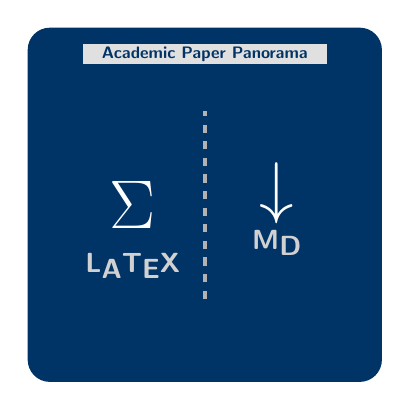
\begin{tikzpicture}

    % 1. 绘制圆角矩形背景 (主体)
    \draw[fill=paperblue, draw=none, rounded corners=8pt] (0,0) rectangle (128pt, 128pt);

    % 2. 绘制左侧：LaTeX 风格的 Sigma (Σ)
    % 采用微微晶莹剔透的效果
    \node (sigma) at (38pt, 64pt) [
        text=white,
        font=\fontsize{75}{0}\selectfont\bfseries\fontfamily{cmr}\selectfont
    ] {$\Sigma$};
    
    % 在 Sigma 下方装饰一个小小的 'LT' (LaTeX)
    \node[below=2pt of sigma, text=grey!30, font=\fontsize{10}{0}\selectfont\sffamily\bfseries] {L\raisebox{-0.5ex}{A}T\raisebox{-0.5ex}{E}X};

    % 3. 绘制中间：代表同步的虚线
    \draw[dashed, grey!50, line width=1.5pt] (64pt, 30pt) -- (64pt, 98pt);

    % 4. 绘制右侧：Markdown 风格的箭头 (↓)
    % 使用经典的 Markdown 标识装饰
    \node (md) at (90pt, 68pt) [
        text=white,
        font=\fontsize{85}{0}\selectfont\bfseries\fontfamily{cmss}\selectfont
    ] {$\downarrow$};

    % 在箭头下方装饰一个小小的 'MD' (Markdown)
    \node[below=-5pt of md, text=grey!30, font=\fontsize{10}{0}\selectfont\sffamily\bfseries] {M\raisebox{-0.5ex}{D}};

    % 5. 绘制顶部的横条：凸显“预览”和“官网”感
    \draw[fill=grey!20, draw=none] (20pt, 115pt) rectangle (108pt, 122pt);
    \node at (64pt, 118.5pt) [
        text=paperblue,
        font=\fontsize{6}{0}\selectfont\sffamily\bfseries\scshape
    ] {Academic Paper Panorama};

\end{tikzpicture}
\end{document}